\documentclass{beamer}

\usepackage{beamerthemesplit}

\title{TorConnect}
\subtitle{An Anonymous P2P Service}
\author{James Lee}
\institute{University of Maryland, Baltimore County}
\date{May 21, 2008}

\begin{document}

\begin{frame}
\titlepage
\end{frame}

\section{Introduction}
\subsection{TorConnect}
\begin{frame}{What is TorConnect?}
\begin{itemize}
\item  TorConnect is an anonymous P2P protocol.
% Based on Direct Connect
% Hub keeps track of users

\pause
\item Uses Tor to hide users' true IP addresses.

\pause
\item Uses Tor hidden services to keep users accessible.

\pause
\item Java hub and client implementation.
\end{itemize}
\end{frame}

\subsection{Motivation}
\begin{frame}{Motivation}
\begin{center}

\includegraphics[width=.9\textwidth]{vfv-crowd.jpg}
\end{center}

\emph{I want to be able to participate in a community anonymously.}

\begin{itemize}
\pause
\item Why would anyone want to remain anonymous?
% Have illegal material.
% Have embarrassing material.
% Fear retribution for sensitive, offensive message.
% Voice opinion.
% Government censorship.

\pause
\item Why participate in a community?
% Meet others with a shared interest.
% Develop friendships. 
% Example: UMBC Hub.

\pause
\item How can we build a new community?
% Must have ability to discover new users.
% Users need reason to join.
% Could be filesharing and chatting.
% UMBC hub not as popular without filesharing.
% Must also be easy to use.

\pause
\item Why use Tor?
% Persistent routes->reduce latency->increasing throughput.
% Largest anonymity network.
% Academically scrutinized.
% Easy application interface with SOCKS and control protocol.
\end{itemize}
\end{frame}

\subsection{Previous Work}
\begin{frame}{Previous Work}
Most work on Tor attempts to make it easier for a single user to access the network.

\begin{columns}
\column{.3\textwidth}
\begin{itemize}
% Examples:
\item<2-> Torbutton, Vidalia
% Torbutton for Firefox.
% Vidalia for generic communication.
% Easy to install; almost no configuration.
% Method for actual communication must be provided some other way.

\item<3-> TorChat
% Clients act like hidden services->16 char pseudonym.
% Chat by connecting to other user by pseudonym.
% Decentralized->not suitable for community. (must already know addr)
% Setup is easy on Windows.
% Manual setup on Linux.

\pause
\item<4-> Direct Connect
% Mention problems.
% Esp. with UMBC hub.


%
% Segue
%
\end{itemize}

\column{.7\textwidth}
\includegraphics<2>[width=\textwidth]{torbutton.png}
\includegraphics<3>[width=\textwidth]{torchat.png}
\includegraphics<4>[width=\textwidth]{dc.png}
\end{columns}
\end{frame}

\section{Design}
\subsection{Handshake}

\begin{frame}{Source Address Discovery}
\begin{itemize}
\item Current P2P systems are designed around IP addressing.
% Example: BitTorrent

\pause
\item Servers can reliably get a client's address from TCP.

\pause
\item This doesn't work on Tor.  How can a Tor service get clients' addresses (psedonyms)?

\pause
\item Just have the client tell the server who they are.

\pause
\item Handshake prevents clients from lying.
\end{itemize}
\end{frame}

\begin{frame}{The Handshaking Process}
\begin{center}
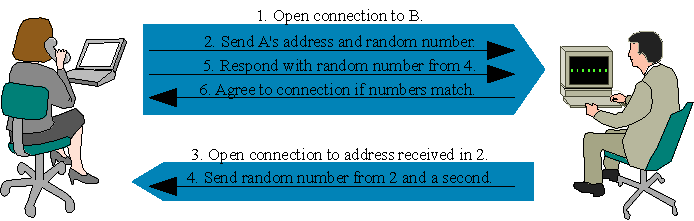
\includegraphics[width=.9\textwidth]{handshake.pdf}
\end{center}
\end{frame}

\subsection{Protocol}
\begin{frame}{The Thing About the Protocol}
After a handshake, you can treat the connection like any other TCP stream.  So you can adapt just about any TCP protocol.
% Proposal called for identifying tokens in every message instead of handshakes.
% After handshaking, any protocol can be used, just replace IP addresses with Tor pseudonyms where applicable.
% Made protocol design a boring exercise.
% Did my best to make it simple to parse and implement and prove my concept in a short period of time.
% Instead focused on robust, generic Tor control, connection libraries which can be used by more mature protocols.
\end{frame}

\subsection{Application}
\begin{frame}{Application Components}
\begin{center}
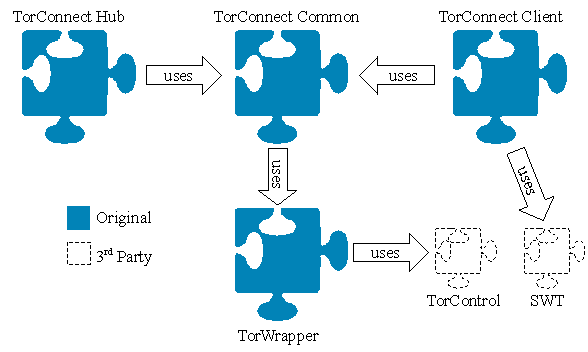
\includegraphics[width=.9\textwidth]{architecture.pdf}
\end{center}
\end{frame}

\section{Analysis}

\subsection{Security}
\begin{frame}{Security}
\begin{block}{Security means:}
\begin{itemize}
\pause
\item It is not possible to determine the actual identity of any user.
\pause
\item Users are the pseudoanonymous identity that they claim.
\end{itemize}
\end{block}

\begin{block}{}
\begin{itemize}
\pause
\item The protocol contains no identifying information
% Does not stop the user from exposing themselves accidentally.

\pause
\item Handshakes really do prevent users from spoofing their identity.
% Suppose a client lies about their identity...

% The only new work I did besides the proto and the handshake was the implementation.
% So any security problems must lie in the implementation or the 3rd party utilities (including Tor itself).
\end{itemize}
\end{block}
\end{frame}

\subsection{Usability}
\begin{frame}{Usability}
\begin{itemize}
\item Software requires no configuration.
\item Software requires no installation.
\item Behaves similar to Direct Connect.
\item However, TorConnect is completely unusable.
% Tor is just too slow.
\end{itemize}
\end{frame}

\subsection{Open Problems}
\begin{frame}{Open Problems}
\begin{itemize}
\item How can speed and reliability be improved?
% Probably can't when relying on volunteers.
% Require participants to run a router?
% Require certain bandwidths?

\pause
\item Use cryptography instead of handshakes.

\pause
\item Adapt a more mature P2P protocol.
% Mine lacks features like pausing, swarming.
\end{itemize}
\end{frame}

\appendix
\section{References}
~\nocite{tor-design}
~\nocite{chaum-mix}
~\nocite{tor-chat}
~\nocite{wiki-spoofing}
~\nocite{tor-control}
~\nocite{tor-ctl}
\bibliographystyle{plainurl}
\bibliography{final-presentation}

\end{document}
